\section{Overview}

The RCO protocol, as defined in the preceding sections, establishes a mathematically rigorous framework for ensuring deterministic, verifiable, and state-consistent telemetry in feedback-coupled systems. However, practical deployment requires the translation of these formal constructs into a concrete system architecture composed of interacting components, communication channels, and execution pipelines.

This section presents a comprehensive architectural model that implements the RCO protocol in a distributed environment. Each mathematical operator introduced in the cryptographic core is mapped to a corresponding system component, and the ingestion pipeline is realized as a sequence of deterministic processing stages. The resulting architecture ensures that the theoretical guarantees of the protocol are preserved under real-world conditions.

\section{Architectural Abstraction}

Let the system be defined as a tuple:

\begin{equation}
\mathcal{A}_{\text{sys}} = (\mathcal{N}, \mathcal{C}, \mathcal{P}, \mathcal{T})
\end{equation}

where:
\begin{itemize}
\item $\mathcal{N}$ is the set of computational nodes,
\item $\mathcal{C}$ is the set of communication channels,
\item $\mathcal{P}$ is the set of processing pipelines,
\item $\mathcal{T}$ is the set of telemetry streams.
\end{itemize}

Each node $N_i \in \mathcal{N}$ executes a deterministic processing function:

\begin{equation}
\mathcal{F}_i: (S_t, D_t, L_{t-1}) \rightarrow (S_{t+1}, L_t)
\end{equation}

subject to the constraints defined by the RCO protocol.

\section{Component Decomposition}

The architecture is decomposed into the following primary components:

\subsection{Telemetry Producers}

Telemetry producers are entities that generate raw telemetry data from system processes, sensors, or computational outputs. Formally, a producer implements:

\begin{equation}
D_t = \mathcal{G}(S_t)
\end{equation}

where $\mathcal{G}$ is the observation function.

Producers are untrusted by default and must not be assumed to generate valid or consistent data.

\subsection{Canonicalization Engine}

The canonicalization engine implements the deterministic serialization function $\mathcal{S}$. Given input telemetry $D_t$, it produces:

\begin{equation}
B_t = \mathcal{S}(D_t)
\end{equation}

This component enforces:
\begin{equation}
D_1 \equiv D_2 \implies B_1 = B_2
\end{equation}

ensuring representation consistency across nodes.

\subsection{Hashing Module}

The hashing module computes the content hash:

\begin{equation}
H_t = \mathcal{H}(B_t)
\end{equation}

This module must use a cryptographically secure hash function with collision resistance properties.

\subsection{Lineage Engine}

The lineage engine maintains the recursive hash chain:

\begin{equation}
L_t = \mathcal{H}(H_t \concat L_{t-1})
\end{equation}

It is responsible for:
\begin{itemize}
\item maintaining temporal ordering,
\item detecting tampering,
\item ensuring continuity of the telemetry sequence.
\end{itemize}

\subsection{State Binding Module}

The state binding module computes:

\begin{equation}
M_t = \mathcal{H}_S(S_t) \concat L_t
\end{equation}

This module ensures that telemetry is cryptographically tied to the system state.

\subsection{Validator Network}

The validator network consists of nodes $\mathcal{V} = \{V_1, \dots, V_n\}$ that independently verify telemetry and generate partial signatures.

Each validator implements:

\begin{equation}
\sigma_i = \text{Sign}_i(M_t, K_i)
\end{equation}

Validators operate under a zero-trust model and must independently verify all conditions.

\subsection{Aggregation Layer}

The aggregation layer collects partial signatures and constructs:

\begin{equation}
\Sigma_t = \text{Aggregate}(\sigma_{i_1}, \dots, \sigma_{i_m})
\end{equation}

for $m \geq t$.

\subsection{Verification Engine}

The verification engine evaluates:

\begin{equation}
\text{Verify}(M_t, \Sigma_t, PK)
\end{equation}

and determines acceptance or rejection of telemetry.

\section{Pipeline Architecture}

The system implements a deterministic pipeline:

\begin{equation}
D_t \rightarrow \mathcal{S} \rightarrow \mathcal{H} \rightarrow \mathcal{C} \rightarrow \mathcal{H}_S \rightarrow \text{Sign} \rightarrow \text{Aggregate} \rightarrow \text{Verify}
\end{equation}

\begin{figure}[htbp]
\centering
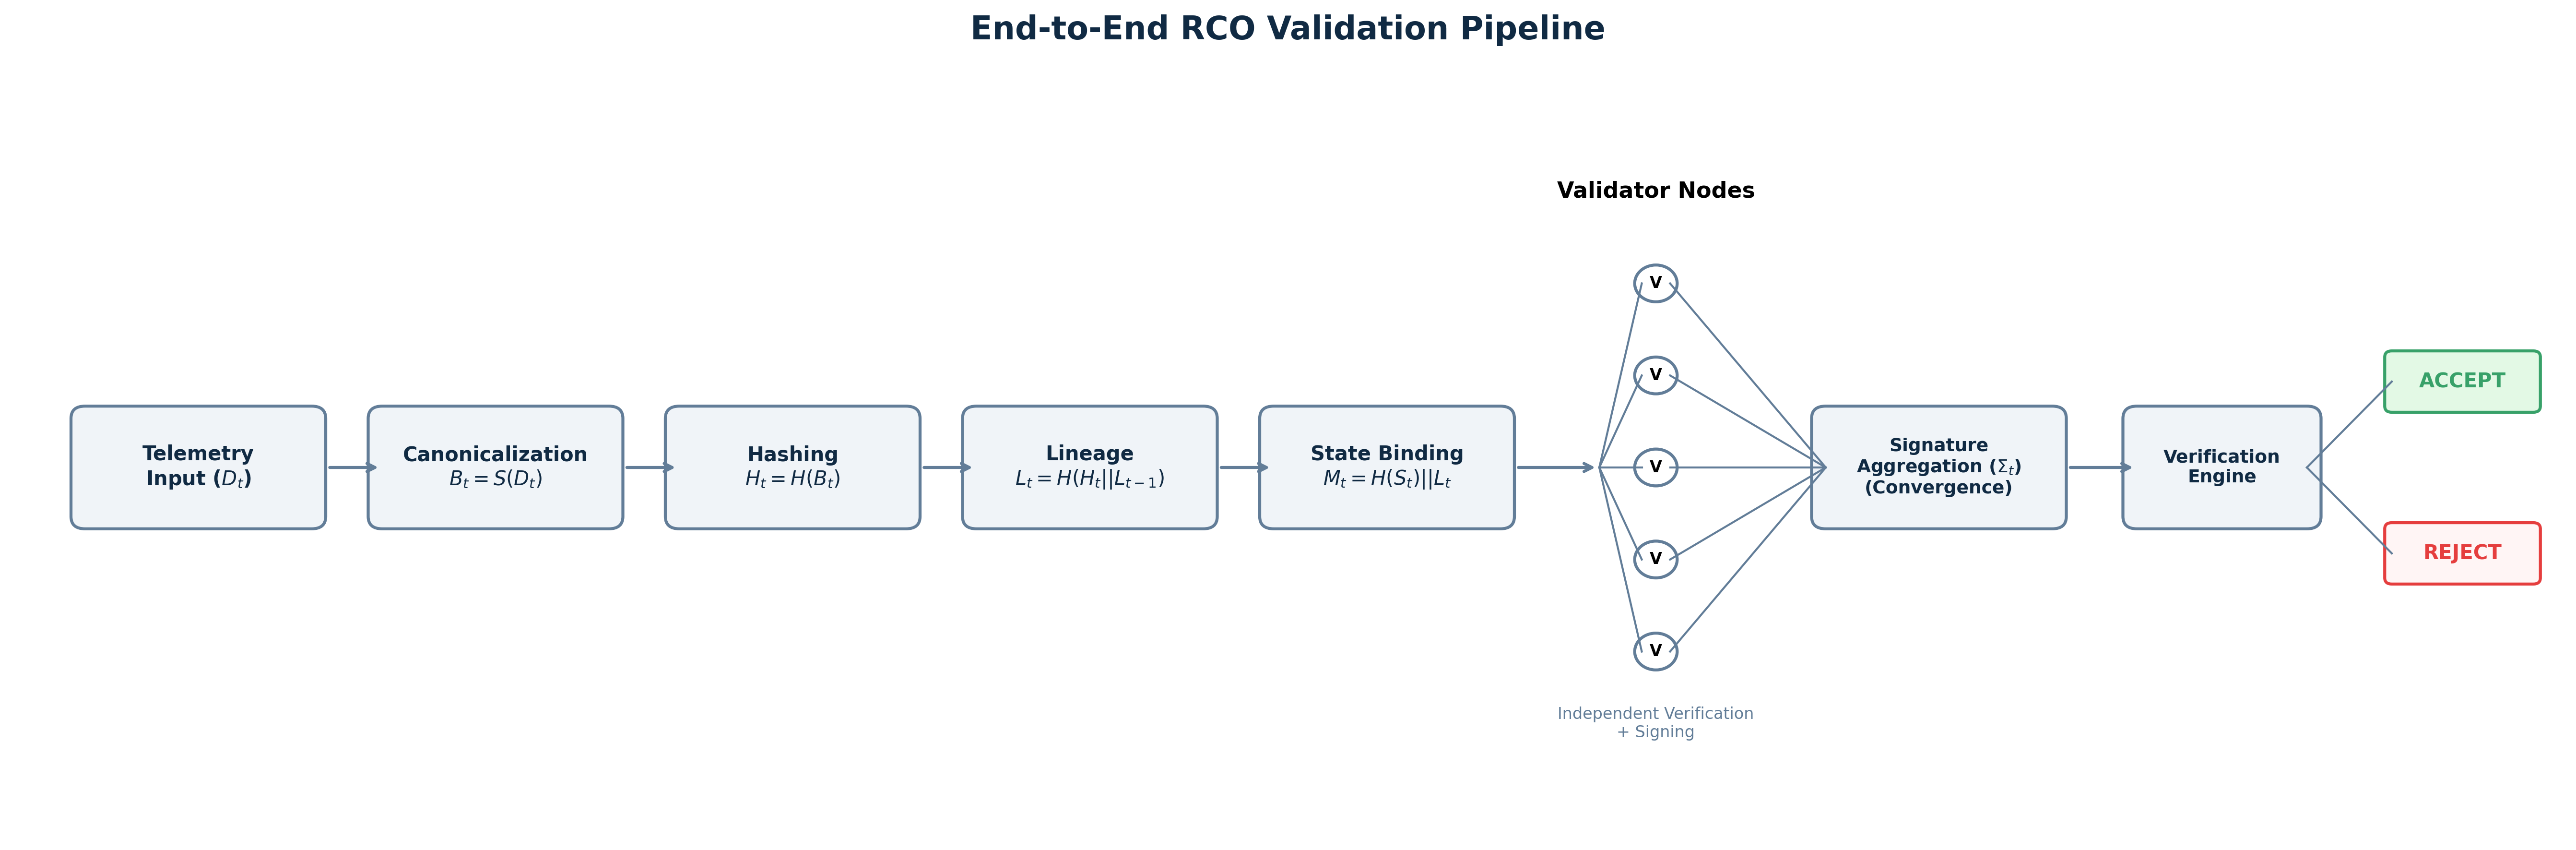
\includegraphics[width=\textwidth]{figures/2-Dimentionals/pipeline_diagram.png}
\caption{End-to-End RCO Validation Pipeline illustrating canonicalization, hashing, lineage construction, state binding, and multi-party validation prior to ingestion.}
\label{fig:pipeline}
\end{figure}

Each stage is stateless with respect to external influence and deterministic given its inputs.

\section{Data Flow Model}

The flow of data through the system is defined as:

\begin{equation}
(D_t, S_t, L_{t-1}) \xrightarrow{\text{pipeline}} (H_t, L_t, \Sigma_t)
\end{equation}

This transformation ensures that each telemetry element is:

\begin{itemize}
\item deterministically encoded,
\item cryptographically hashed,
\item chained into lineage,
\item bound to system state,
\item verified by multiple validators.
\end{itemize}

\section{Distributed Deployment Model}

The architecture supports distributed deployment across multiple nodes. Let $\mathcal{N}$ be partitioned into:

\begin{equation}
\mathcal{N} = \mathcal{N}_{\text{producers}} \cup \mathcal{N}_{\text{validators}} \cup \mathcal{N}_{\text{consumers}}
\end{equation}

Each node type performs distinct roles:

\begin{itemize}
\item Producers generate telemetry,
\item Validators verify and sign,
\item Consumers use validated telemetry.
\end{itemize}

\section{Consistency Across Nodes}

All nodes must maintain identical lineage state:

\begin{equation}
\forall i,j, \quad L_t^{(i)} = L_t^{(j)}
\end{equation}

This is ensured through deterministic processing and consensus on accepted telemetry.

\section{Fault Tolerance}

The system tolerates up to $f < t$ faulty validators. If fewer than $t$ signatures are available, telemetry is rejected, preserving safety.

\section{Scalability Considerations}

The architecture supports horizontal scaling:

\begin{equation}
\text{Throughput} \propto |\mathcal{V}|
\end{equation}

as signature generation and verification can be parallelized.

\section{Conclusion}

The system architecture presented in this section provides a direct mapping from the formal RCO model to a deployable infrastructure. By decomposing the protocol into well-defined components and enforcing deterministic processing at each stage, the architecture preserves the integrity guarantees established in the cryptographic and security analyses while enabling practical implementation in distributed environments.

\section{Pipeline Execution and Sequence Semantics}

The RCO architecture is realized as a deterministic execution pipeline in which telemetry data flows through a sequence of transformation and verification stages. Each stage enforces a specific invariant and produces an output that serves as the input to the next stage. The correctness of the system depends on the strict ordering and deterministic execution of these stages across all participating nodes.

\subsection{Execution Model}

Let a telemetry event be represented as a tuple:

\begin{equation}
E_t = (D_t, S_t, L_{t-1})
\end{equation}

The pipeline execution is defined as a sequence of transformations:

\begin{equation}
E_t \xrightarrow{\mathcal{S}} B_t \xrightarrow{\mathcal{H}} H_t \xrightarrow{\mathcal{C}} L_t \xrightarrow{\mathcal{H}_S} M_t \xrightarrow{\text{Sign}} \{\sigma_i\} \xrightarrow{\text{Aggregate}} \Sigma_t \xrightarrow{\text{Verify}} \text{Decision}
\end{equation}

Each transformation is deterministic and side-effect-free with respect to external state.

\subsection{Stage-by-Stage Execution Semantics}

\paragraph{Stage 1: Canonicalization}

\begin{equation}
B_t = \mathcal{S}(D_t)
\end{equation}

The system enforces:
\begin{equation}
\forall i,j, \quad \mathcal{S}_i(D_t) = \mathcal{S}_j(D_t)
\end{equation}

ensuring cross-node consistency.

\paragraph{Stage 2: Hashing}

\begin{equation}
H_t = \mathcal{H}(B_t)
\end{equation}

This stage compresses the telemetry into a fixed-length representation.

\paragraph{Stage 3: Lineage Update}

\begin{equation}
L_t = \mathcal{H}(H_t \concat L_{t-1})
\end{equation}

This enforces temporal ordering and immutability.

\paragraph{Stage 4: State Binding}

\begin{equation}
M_t = \mathcal{H}_S(S_t) \concat L_t
\end{equation}

This binds telemetry to system state.

\paragraph{Stage 5: Distributed Signing}

Each validator computes:

\begin{equation}
\sigma_i = \text{Sign}_i(M_t, K_i)
\end{equation}

\paragraph{Stage 6: Aggregation}

\begin{equation}
\Sigma_t = \text{Aggregate}(\sigma_{i_1}, \dots, \sigma_{i_m})
\end{equation}

\paragraph{Stage 7: Verification}

\begin{equation}
\text{Decision} =
\begin{cases}
\text{accept}, & \text{if } \text{Verify}(M_t, \Sigma_t, PK) \\
\text{reject}, & \text{otherwise}
\end{cases}
\end{equation}

\subsection{End-to-End Execution Invariant}

The pipeline enforces:

\begin{equation}
\text{accept}(E_t) \implies \text{Valid}(D_t)
\end{equation}

ensuring that only valid telemetry progresses.

\section{Sequence Diagram Representation}

The interaction between components may be represented as a sequence diagram. The following LaTeX-compatible representation describes the interaction flow.

\subsection{Logical Sequence Description}

\begin{equation}
\text{Producer} \rightarrow \text{Canonicalizer} \rightarrow \text{Hasher} \rightarrow \text{Lineage Engine} \rightarrow \text{Validators} \rightarrow \text{Aggregator} \rightarrow \text{Verifier}
\end{equation}

\subsection{Formal Interaction Steps}

\begin{enumerate}
\item Producer emits $D_t$
\item Canonicalizer computes $B_t = \mathcal{S}(D_t)$
\item Hasher computes $H_t = \mathcal{H}(B_t)$
\item Lineage engine computes $L_t$
\item State binding computes $M_t$
\item Validators receive $(M_t)$ and produce $\sigma_i$
\item Aggregator collects $\sigma_i$ and computes $\Sigma_t$
\item Verifier evaluates $\Sigma_t$ and returns decision
\end{enumerate}

\subsection{TikZ Sequence Diagram Template}

The following structure can be used to render diagrams:

\begin{verbatim}
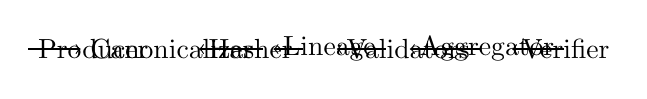
\begin{tikzpicture}
\node (producer) {Producer};
\node (canon) [right of=producer] {Canonicalizer};
\node (hash) [right of=canon] {Hasher};
\node (lineage) [right of=hash] {Lineage};
\node (validators) [right of=lineage] {Validators};
\node (agg) [right of=validators] {Aggregator};
\node (verify) [right of=agg] {Verifier};

\draw[->] (producer) -- (canon);
\draw[->] (canon) -- (hash);
\draw[->] (hash) -- (lineage);
\draw[->] (lineage) -- (validators);
\draw[->] (validators) -- (agg);
\draw[->] (agg) -- (verify);
\end{tikzpicture}
\end{verbatim}

\section{Real-World Deployment Topologies}

The RCO architecture is designed to operate across multiple deployment environments, including centralized cloud systems, decentralized edge networks, and hybrid configurations.

\begin{figure}[htbp]
\centering
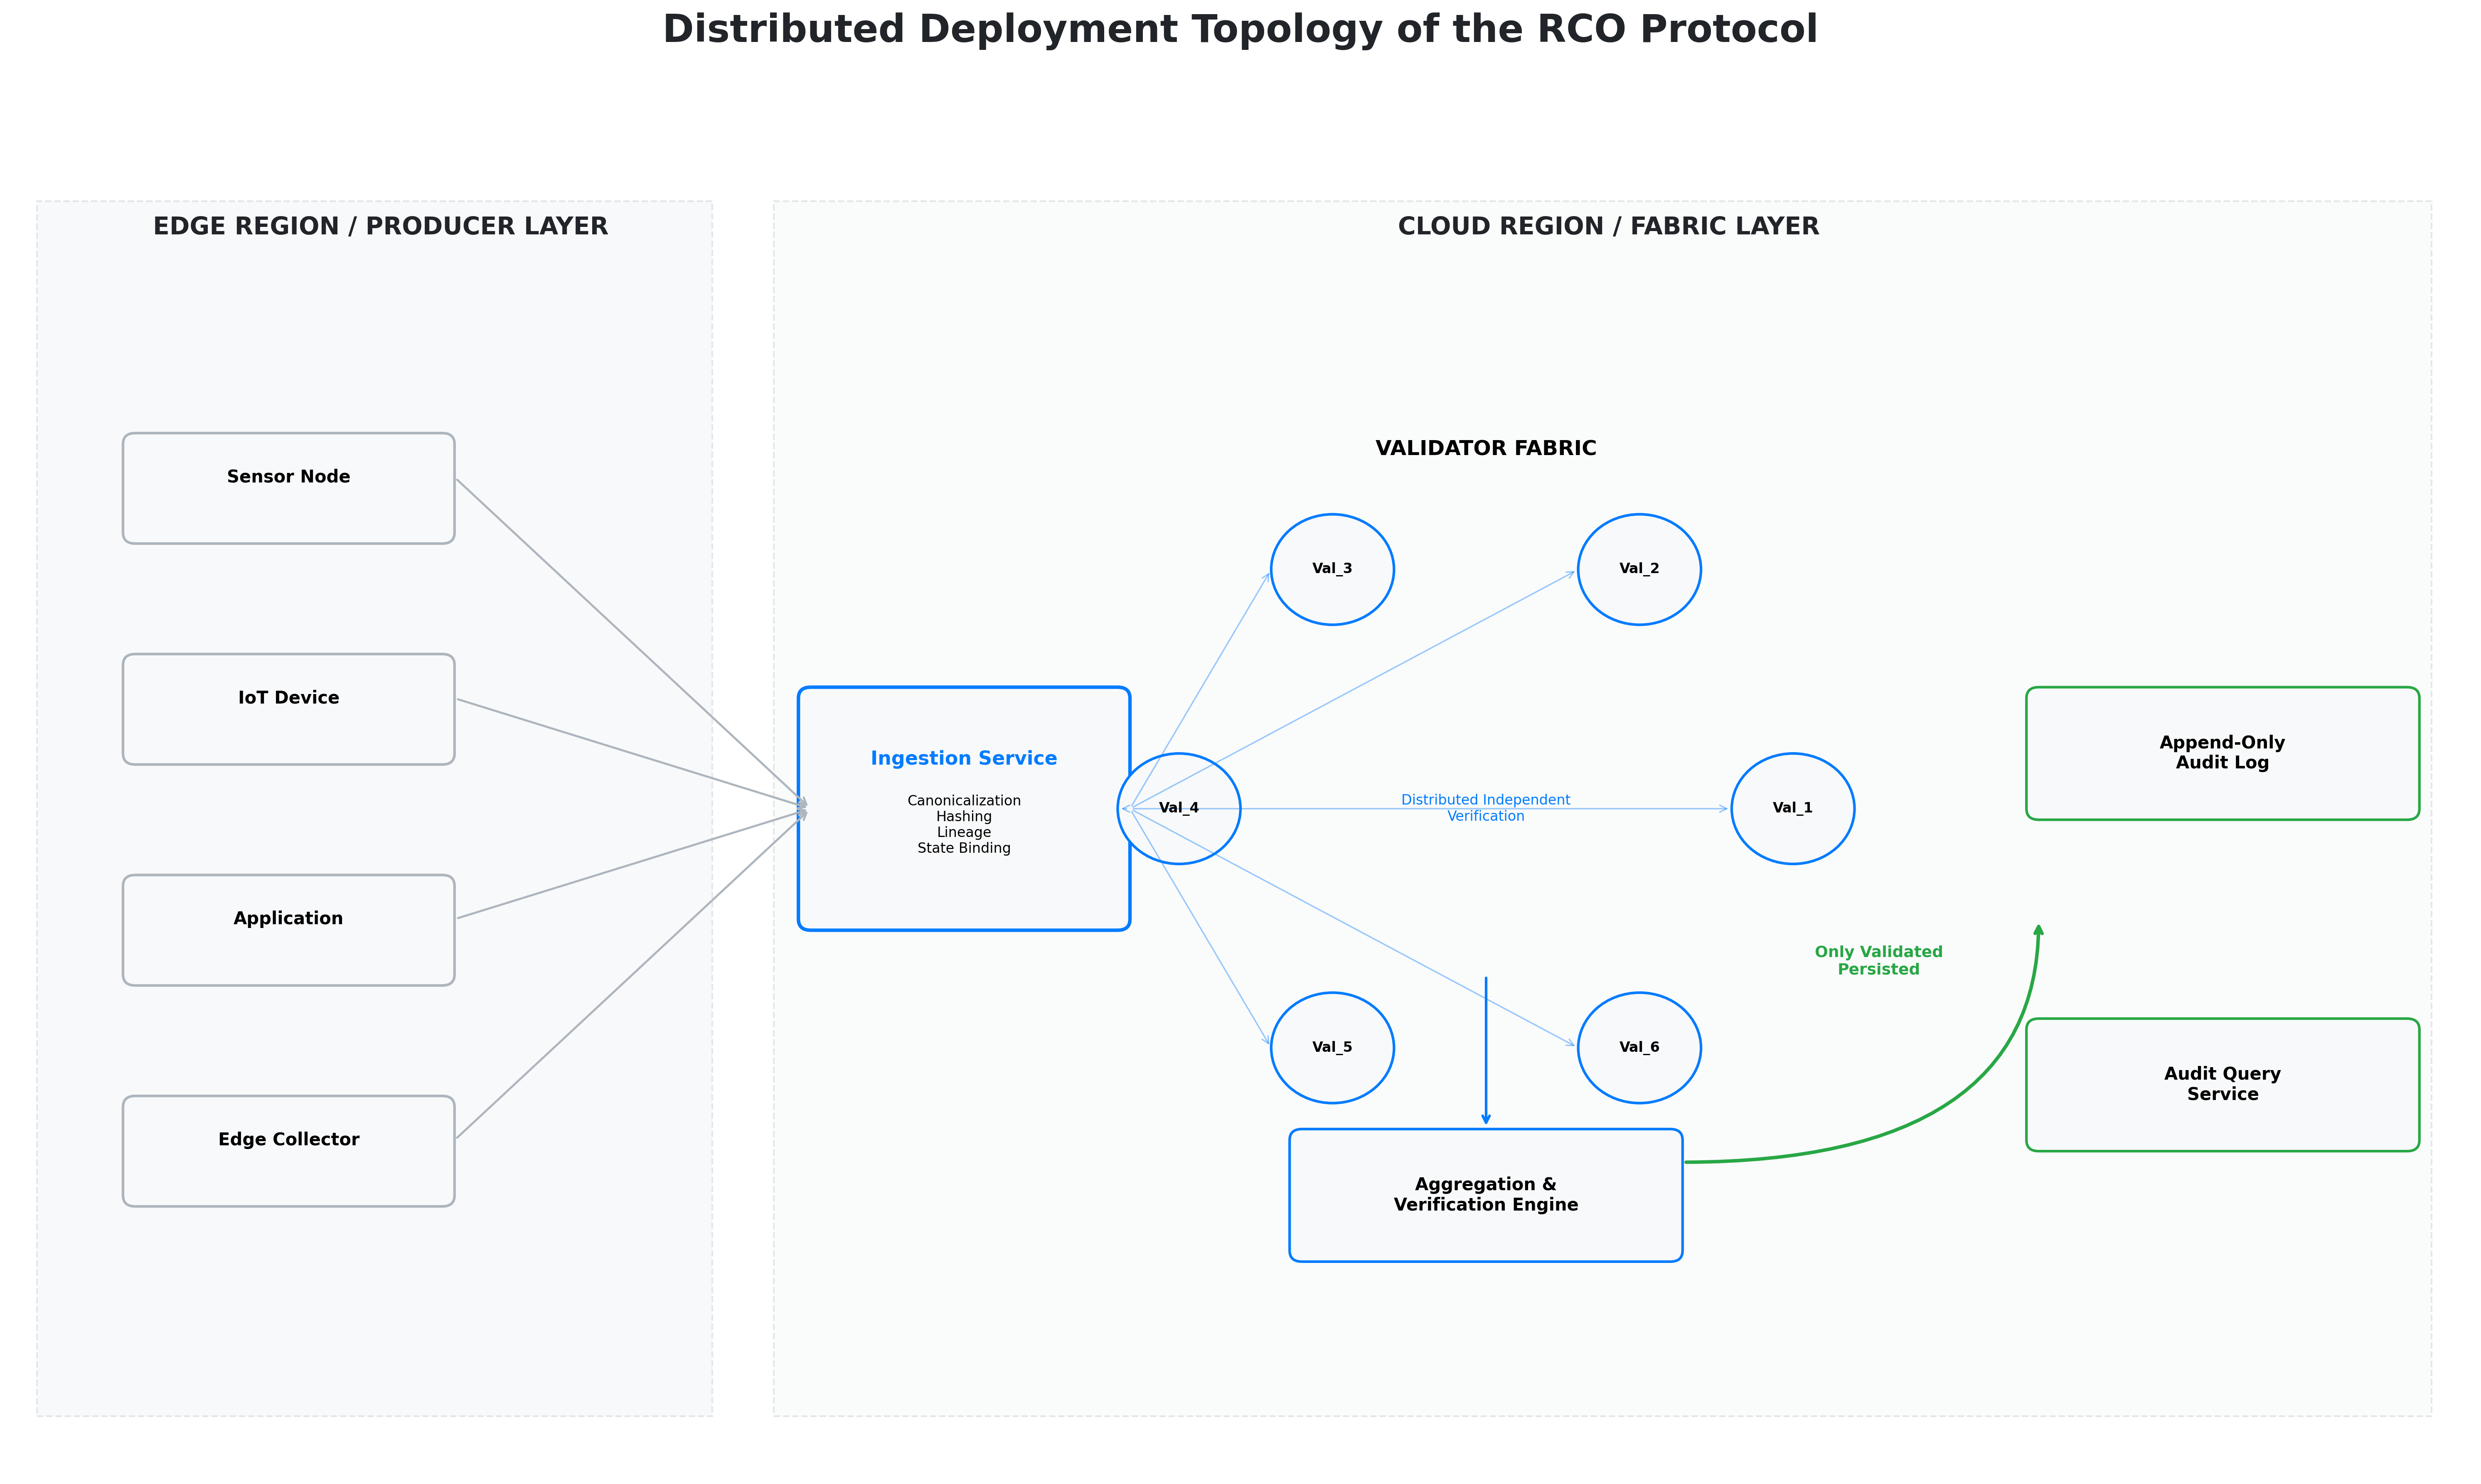
\includegraphics[width=\textwidth]{figures/2-Dimentionals/deployment_topology.png}
\caption{Distributed deployment topology across edge and cloud environments, illustrating producers, ingestion layer, validator fabric, and storage systems.}
\label{fig:deployment}
\end{figure}

\subsection{Cloud Deployment Model}

In a cloud deployment, all components are hosted within a centralized infrastructure:

\begin{equation}
\mathcal{N} = \mathcal{N}_{\text{cloud}}
\end{equation}

Characteristics:
\begin{itemize}
\item Low latency between components
\item High computational resources
\item Centralized management
\end{itemize}

Validators may be deployed as independent services within the cloud to preserve zero-trust properties.

\subsection{Edge Deployment Model}

In an edge deployment, telemetry producers and validators are distributed across geographically dispersed nodes:

\begin{equation}
\mathcal{N} = \mathcal{N}_{\text{edge}}
\end{equation}

Characteristics:
\begin{itemize}
\item Reduced latency to data sources
\item Increased network variability
\item Partial connectivity
\end{itemize}

The ingestion pipeline must handle intermittent connectivity and delayed aggregation.

\subsection{Hybrid Deployment Model}

A hybrid model combines cloud and edge components:

\begin{equation}
\mathcal{N} = \mathcal{N}_{\text{edge}} \cup \mathcal{N}_{\text{cloud}}
\end{equation}

In this model:
\begin{itemize}
\item Canonicalization and hashing occur at the edge,
\item Aggregation and verification occur in the cloud,
\item Lineage is synchronized across both layers.
\end{itemize}

\subsection{Topology Selection Criteria}

The choice of deployment topology depends on:

\begin{equation}
\text{Topology} = f(\text{latency}, \text{throughput}, \text{trust}, \text{connectivity})
\end{equation}

\subsection{Distributed Validator Placement}

Validators should be distributed such that:

\begin{equation}
\forall i,j, \quad \text{NetworkDistance}(V_i, V_j) \text{ is maximized}
\end{equation}

to reduce correlated failures and collusion risk.

\subsection{Scalability Model}

Let $n$ be the number of validators. The system throughput is:

\begin{equation}
\text{Throughput} = O(n)
\end{equation}

while verification cost remains constant due to aggregation.

\subsection{Fault Isolation}

Failures in one component do not propagate:

\begin{equation}
\text{Failure}(C_i) \not\implies \text{Failure}(C_j)
\end{equation}

for $i \neq j$, ensuring modular resilience.

\subsection{Deployment Invariant}

Regardless of topology, the system must enforce:

\begin{equation}
\forall t, \quad L_t^{(i)} = L_t^{(j)}
\end{equation}

across all nodes.

\section{Conclusion}

The pipeline execution model and deployment topologies described in this section translate the formal RCO protocol into a concrete, implementable system. By defining deterministic execution semantics, explicit interaction flows, and flexible deployment configurations, the architecture ensures that the theoretical guarantees of the protocol are preserved in practical environments. This establishes a foundation for building scalable, secure, and verifiable telemetry systems across diverse infrastructure settings.

\section{API Design, Data Structures, Storage Model, and Performance Analysis}

The practical deployment of the RCO protocol requires a well-defined interface layer through which telemetry producers, validators, and consumers interact with the system. This section specifies the application programming interfaces (APIs), internal data structures, storage mechanisms, and performance characteristics necessary to implement the protocol in production environments.

\section{API Design}

The API layer provides a deterministic interface for submitting telemetry, retrieving lineage states, and verifying proofs.

\subsection{Telemetry Submission API}

The primary entry point into the system is the telemetry submission endpoint:

\begin{equation}
\texttt{SubmitTelemetry}(D_t, S_t) \rightarrow (L_t, \Sigma_t, \text{status})
\end{equation}

The function executes the full ingestion pipeline:

\begin{equation}
(D_t, S_t, L_{t-1}) \rightarrow (H_t, L_t, \Sigma_t)
\end{equation}

The response includes:
\begin{itemize}
\item $L_t$: updated lineage state,
\item $\Sigma_t$: aggregated proof,
\item status: accept or reject.
\end{itemize}

\subsection{Verification API}

External entities may verify telemetry independently:

\begin{equation}
\texttt{VerifyTelemetry}(D_t, S_t, L_{t-1}, \Sigma_t) \rightarrow \{\text{true}, \text{false}\}
\end{equation}

This API recomputes:

\begin{equation}
B_t = \mathcal{S}(D_t), \quad H_t = \mathcal{H}(B_t), \quad L_t = \mathcal{H}(H_t \concat L_{t-1})
\end{equation}

and verifies:

\begin{equation}
\text{Verify}(\mathcal{H}_S(S_t) \concat L_t, \Sigma_t, PK)
\end{equation}

\subsection{Lineage Query API}

\begin{equation}
\texttt{GetLineage}(t) \rightarrow L_t
\end{equation}

This allows retrieval of lineage states for auditing.

\subsection{Batch Processing API}

For high-throughput environments:

\begin{equation}
\texttt{SubmitBatch}(\{D_i, S_i\}_{i=1}^{k}) \rightarrow \{(L_i, \Sigma_i)\}_{i=1}^{k}
\end{equation}

Batch processing preserves ordering:

\begin{equation}
L_i = \mathcal{H}(H_i \concat L_{i-1})
\end{equation}

\section{Data Structures}

The system maintains several core data structures.

\subsection{Telemetry Record}

\begin{equation}
\mathcal{R}_t = (D_t, B_t, H_t, L_t, \Sigma_t)
\end{equation}

This structure encapsulates all information required for verification.

\subsection{Lineage Chain}

The lineage is stored as a sequence:

\begin{equation}
\mathcal{L} = \{L_0, L_1, \dots, L_t\}
\end{equation}

Each element depends on its predecessor.

\subsection{Validator State}

Each validator maintains:

\begin{equation}
\mathcal{V}_i = (K_i, PK, \text{local cache})
\end{equation}

\subsection{Proof Object}

\begin{equation}
\Sigma_t = (\sigma_{i_1}, \dots, \sigma_{i_m})
\end{equation}

or its aggregated form.

\section{Storage Model}

The storage layer must ensure persistence, immutability, and efficient retrieval.

\subsection{Append-Only Log}

Telemetry records are stored in an append-only log:

\begin{equation}
\mathcal{S}_{\text{log}} = [\mathcal{R}_0, \mathcal{R}_1, \dots, \mathcal{R}_t]
\end{equation}

This ensures immutability:

\begin{equation}
\forall i < j, \quad \mathcal{R}_i \text{ cannot be modified after } \mathcal{R}_j \text{ is written}
\end{equation}

\subsection{Indexing}

Efficient lookup is enabled via indexing:

\begin{equation}
\text{Index}: t \mapsto \mathcal{R}_t
\end{equation}

\subsection{Distributed Storage}

In distributed environments:

\begin{equation}
\mathcal{S}_{\text{dist}} = \bigcup_{i=1}^{n} \mathcal{S}_i
\end{equation}

Each node stores a replica of the log.

\subsection{Consistency Model}

The system enforces strong consistency:

\begin{equation}
\forall i,j, \quad \mathcal{S}_i = \mathcal{S}_j
\end{equation}

subject to eventual synchronization.

\subsection{Checkpointing}

To reduce storage overhead, checkpoints may be introduced:

\begin{equation}
C_k = L_k
\end{equation}

allowing reconstruction from checkpoints.

\section{Memory Model}

The system uses:

\begin{itemize}
\item In-memory buffers for pending telemetry,
\item Persistent storage for finalized records,
\item Caches for frequently accessed lineage states.
\end{itemize}

\section{Performance Characteristics}

\subsection{Time Complexity}

For each telemetry element:

\begin{equation}
T_{\text{total}} = T_{\mathcal{S}} + T_{\mathcal{H}} + T_{\mathcal{C}} + T_{\text{sign}} + T_{\text{agg}} + T_{\text{verify}}
\end{equation}

Where:
\begin{itemize}
\item $T_{\mathcal{S}} = O(n \log n)$ for sorting keys,
\item $T_{\mathcal{H}} = O(|B_t|)$,
\item $T_{\mathcal{C}} = O(1)$,
\item $T_{\text{sign}} = O(1)$ per validator,
\item $T_{\text{agg}} = O(t)$,
\item $T_{\text{verify}} = O(1)$.
\end{itemize}

Thus:

\begin{equation}
T_{\text{total}} = O(n \log n + |B_t| + t)
\end{equation}

\subsection{Space Complexity}

\begin{equation}
S_{\text{total}} = O(t \cdot k)
\end{equation}

where $k$ is hash size.

\subsection{Network Complexity}

Each telemetry requires:

\begin{equation}
O(n) \text{ messages for signature distribution}
\end{equation}

\subsection{Latency Model}

\begin{equation}
T_{\text{latency}} = \max_i T_{\text{sign}}^{(i)} + T_{\text{network}} + T_{\text{agg}}
\end{equation}

\subsection{Throughput}

\begin{equation}
\text{Throughput} \propto \frac{1}{T_{\text{latency}}}
\end{equation}

\section{Optimization Strategies}

\subsection{Parallel Signing}

Validators operate in parallel:

\begin{equation}
T_{\text{sign}} = \max_i T_{\text{sign}}^{(i)}
\end{equation}

\subsection{Batch Aggregation}

\begin{equation}
\Sigma = \text{Aggregate}(\{\sigma_i^{(j)}\})
\end{equation}

for multiple $j$.

\subsection{Caching}

\begin{equation}
\text{Cache}(L_t) \rightarrow O(1) \text{ retrieval}
\end{equation}

\section{Scalability Analysis}

Let $n$ be validators and $t$ threshold.

\begin{equation}
\text{Scalability} = O(n) \quad \text{(parallelizable)}
\end{equation}

Verification remains constant due to aggregation.

\section{Fault Tolerance}

The system tolerates:

\begin{equation}
f < t
\end{equation}

faulty validators.

\section{Deployment Constraints}

\begin{equation}
\text{Consistency} > \text{Availability}
\end{equation}

ensuring safety-first design.

\section{End-to-End Performance Bound}

\begin{equation}
\Pr[\text{Failure}] \leq \epsilon_{\mathcal{H}} + \epsilon_{\mathcal{H}_S} + \epsilon_{\text{sig}} + \epsilon_{\text{threshold}}
\end{equation}

\section{Conclusion}

This section defines a complete production-ready specification for implementing the RCO protocol. By formalizing APIs, data structures, storage models, and performance characteristics, it bridges the gap between theoretical design and practical deployment. The architecture ensures that the integrity guarantees established in earlier sections are preserved while enabling scalable and efficient operation in real-world environments.